\documentclass{standalone}
\usepackage[dvipsnames,svgnames,x11names]{xcolor}
\usepackage{tikz}
\usepackage{pgfplots}
\pgfplotsset{compat = 1.12}
\usepackage{../thesismath}
\begin{document}
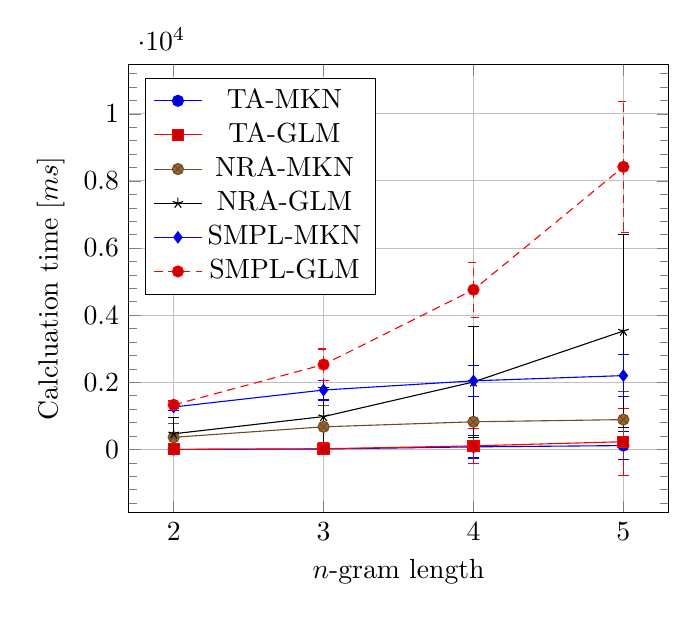
\begin{tikzpicture}[baseline]

\begin{axis}[
  xlabel = {$n$-gram length},
  xtick = {2, ..., 5},
  ylabel = {Calcluation time [$m s$]},
  minor y tick num = 4,
  grid = major,
  legend entries = {{TA-MKN}, {TA-GLM}, {NRA-MKN}, {NRA-GLM}, {SMPL-MKN}, {SMPL-GLM}},
  legend pos = north west,
]

% over 100 test sequences on my own machine

% TA-MKN
\addplot+[
  error bars/.cd,
  y dir = both,
  y explicit,
] table [y error = us_error] {
  n us       us_error
  2    1.015    4.048
  3   12.717  109.787
  4   76.459  332.252
  5  114.836  419.295
};

% TA-GLM
\addplot+[
  error bars/.cd,
  y dir = both,
  y explicit,
] table [y error = us_error] {
  n us       us_error
  2    0.848    3.682
  3   19.619  182.865
  4  105.726  515.667
  5  230.042  996.778
};

% NRA-MKN
\addplot+[
  error bars/.cd,
  y dir = both,
  y explicit,
] table [y error = us_error] {
  n us       us_error
  2  361.671  409.717
  3  673.728  625.481
  4  823.564  761.876
  5  888.625  843.348
};

% NRA-GLM
\addplot+[
  error bars/.cd,
  y dir = both,
  y explicit,
] table [y error = us_error] {
  n us       us_error
  2  466.266  472.377
  3  978.883  879.374
  4 2010.334 1653.606
  5 3528.125 2875.406
};

% SMPL-MKN
\addplot+[
  error bars/.cd,
  y dir = both,
  y explicit,
] table [y error = us_error] {
  n us       us_error
  2 1264.878  114.583
  3 1769.972  296.445
  4 2043.639  464.830
  5 2200.023  627.065
};

% SMPL-GLM
\addplot+[
  error bars/.cd,
  y dir = both,
  y explicit,
] table [y error = us_error] {
  n us       us_error
  2 1328.259  114.931
  3 2528.827  465.161
  4 4758.322  818.769
  5 8419.606 1945.688
};

\end{axis}

\end{tikzpicture}
\end{document}
